% !TeX spellcheck = de_DE
\PassOptionsToPackage{table}{xcolor}
%\documentclass[oneside, english, draft]{sdqthesis}
\documentclass[oneside, german, final]{sdqthesis}


%% ---------------------------------
%% | Information about the thesis  |
%% ---------------------------------

%% Name of the author
\author{Niko Benkler}

%% Title (and possibly subtitle) of the thesis
\title{Testbench for Evaluating Auto-Scalers}

%% Type of the thesis 
\thesistype{Praktikum: Werkzeuge für Agile Modellierung}

%% Change the institute here, ``IPD'' is default
% \myinstitute{Institute for \dots}

%% You can put a logo in the ``logos'' directory and include it here
%% instead of the SDQ logo
% \grouplogo{myfile}
%% Alternatively, you can disable the group logo
% \nogrouplogo

%% The reviewers are the professors that grade your thesis

\advisorone{M.Sc. Manuel Gotin}




\settitle

%% --------------------------------
%% | Settings for word separation |
%% --------------------------------

%% Describe separation hints here.
%% For more details, see 
%% http://en.wikibooks.org/wiki/LaTeX/Text_Formatting#Hyphenation
\hyphenation{
% me-ta-mo-del
}

%% --------------------------------
%% | Bibliography                 |
% --------------------------------

%% Use biber instead of BibTeX, see README
\usepackage[citestyle=numeric,style=numeric,backend=biber]{biblatex}
\addbibresource{Ausarbeitung.bib}


\usepackage[T1]{fontenc}
\usepackage[table]{xcolor}    % loads also »colortbl«
\usepackage{makecell}
\usepackage{adjustbox}
\usepackage{tabularx} % in the preamble
\usepackage{pdflscape}
\usepackage{afterpage}
\usepackage{capt-of}
\usepackage{threeparttable}
\usepackage{listings,xcolor}
\usepackage{graphicx}
\usepackage{pdfpages}
\usepackage{booktabs}
\usepackage{placeins}
\usepackage{float}
\usepackage{pgfgantt}
\usepackage{hyperref}
\usepackage{rotating}
\usepackage{multicol}
\usepackage{makecell}
\usepackage{array,ragged2e}

\colorlet{punct}{red!60!black}
\definecolor{background}{HTML}{EEEEEE}
\definecolor{delim}{RGB}{20,105,176}
\colorlet{numb}{magenta!60!black}

\lstdefinelanguage{json}{
	basicstyle=\normalfont\ttfamily,
	numbers=left,
	numberstyle=\scriptsize,
	stepnumber=1,
	numbersep=8pt,
	showstringspaces=false,
	breaklines=true,
	frame=lines,
	backgroundcolor=\color{background},
	literate=
	*{0}{{{\color{numb}0}}}{1}
	{1}{{{\color{numb}1}}}{1}
	{2}{{{\color{numb}2}}}{1}
	{3}{{{\color{numb}3}}}{1}
	{4}{{{\color{numb}4}}}{1}
	{5}{{{\color{numb}5}}}{1}
	{6}{{{\color{numb}6}}}{1}
	{7}{{{\color{numb}7}}}{1}
	{8}{{{\color{numb}8}}}{1}
	{9}{{{\color{numb}9}}}{1}
	{:}{{{\color{punct}{:}}}}{1}
	{,}{{{\color{punct}{,}}}}{1}
	{\{}{{{\color{delim}{\{}}}}{1}
	{\}}{{{\color{delim}{\}}}}}{1}
	{[}{{{\color{delim}{[}}}}{1}
	{]}{{{\color{delim}{]}}}}{1},
}

\definecolor{dkgreen}{rgb}{0,0.6,0}
\definecolor{gray}{rgb}{0.5,0.5,0.5}
\definecolor{mauve}{rgb}{0.58,0,0.82}
\lstset{frame=tb,
	language=Java,
	aboveskip=3mm,
	belowskip=3mm,
	showstringspaces=false,
	columns=flexible,
	backgroundcolor=\color{background},
	basicstyle={\small\ttfamily},
	numbers=left,
	numberstyle=\scriptsize,
	stepnumber=1,
	numbersep=8pt,
	keywordstyle=\color{blue},
	commentstyle=\color{dkgreen},
	stringstyle=\color{mauve},
	breaklines=true,
	breakatwhitespace=true,
	tabsize=3
}





%% ====================================
%% ====================================
%% ||                                ||
%% || Beginning of the main document ||
%% ||                                ||
%% ====================================
%% ====================================
\begin{document}


%% Set PDF metadata
\setpdf

%% Set the title
\maketitle

%% The Preamble begins here
\frontmatter


\setcounter{page}{1}
\pagenumbering{roman}

%% ----------------
%% |   Abstract   |
%% ----------------
%% For theses written in English, an abstract both in English
%% and German is mandatory.
%%
%% For theses written in German, a German abstract is sufficient.
%%
%% The text is included from the following files:
%% - sections/abstract



%% ------------------------
%% |   Table of Contents  |
%% ------------------------
\tableofcontents

\listoffigures
%\listoftables

%% -----------------
%% |   Main part   |
%% -----------------

\mainmatter


\chapter{Einführung}
\label{ch:Introduction}
Der Aufstieg des Cloud Computing ermöglicht Kunden ihre Applikationen dynamisch zu skalieren. Dies steigert nicht nur die Verfügbarkeit für den Endnutzer, sondern hat auch ökologische und ökonomische Vorteile. Investitionen in Hardware und Software können reduziert werden, da die Ressourcennutzung durch das dynamische Skalieren optimiert wird. Gleichzeitig kann der Klimafußabdruck reduziert werden, da Ressourcen nicht unnötig brach liegen \cite{ASurveyOn} \cite{ReviewOfAtuoScaling}. \\
Trotz dieser Vorteile ist es eine nicht triviale Aufgabe, die korrekte Allokation von Ressourcen zu planen, vorherzusagen und auszuführen. Gründe dafür sind die verschiedenen Charakteristiken der Workloads im Cloud Computing, wie beispielsweise Varianz, Periodizität (Muster, die sich täglich, wöchentlich etc. wiederholen), Art der benötigten Ressource oder Änderungsrate \cite{PEAS}. \\  
Diese Aufgabe wird mittels Auto-Skalierer durchgeführt, die basierend auf der Systemlast, diversen Metriken und Strategien dynamisch Ressourcen hinzufügen oder wieder wegnehmen. Zwischen dem Cloud Service Anbieter und dem Kunden existiert dabei ein Rahmenvertrag (Service Level Agreements oder kurz, \textit{SLAs}), der die Dienstgüte des Cloud Service beschreibt \cite{ASurveyOn}. Dieser Vertrag beschreibt Qualitätsparameter wie Verfügbarkeit, Reaktionszeit des Anbieters, Durchsatz oder die Ausfallrate der Infrastruktur. Der Auto-Skalierer sollte dabei so arbeiten, dass er diese Parameter erfüllt und dabei die Gesamtkosten gering hält, sodass der Anbieter mit seiner angebotenen Leistung Profit erzielen kann. \\
In den letzten Jahren wurden deswegen verschiedenste Strategien für Auto-Skalierer entwickelt, die diese Aufgabe effizient lösen sollen \cite{ReviewOfAtuoScaling}. Um konkrete Implementierungen dieser Auto-Skalierer zu evaluieren, kann man diese auf realer Infrastruktur und unter einer gegebenen Last testen. Dies jedoch erfordert hohe Kosten, da eine Infrastruktur bereitgestellt und eine Last erzeugt werden muss, um so das Verhalten des Auto-Skalieres zu beobachten. Bei einer Simulation hingegen können diese Kosten größtenteils reduziert werden, da nur Ressourcen für die Durchführung der Simulation benötigt werden.\\
Um eine solche Simulation durchzuführen muss eine Umgebung geschaffen werden, in der die Infrastruktur eines Cloud-Service Anbieters modelliert wird, um so das Verhalten eines gegebenen Auto-Skalierers zu beobachten. Diese Entwicklung einer solchen Umgebung, auch Testbench für Auto-Skalierer genannt, ist der Bestandteil dieses Praktikums und wird in der folgenden Dokumentation beschrieben.


\section{Motivation}
\label{sec:Introduction:Motivation}
Bei einer zeit-diskrete Simulationen ist es möglich, das Verhalten eines Auto-Skalierers anhand einer gegebenen diskreten Last auf einer simulierten Infrastruktur zu testen. Dabei kann die diskretisierte Last sowohl auf einer realen Last basieren, die über einen sehr langen Zeitraum gemessen wurde, als auch auf einer generierten Last, die verschiedene, der in der Einführung beschriebenen Charakteristika aufweist. Es ist daher möglich, den Auto-Skalierer ohne größere Anstrengungen unter verschiedenen Lastbedingungen zu testen. Außerdem soll eine Testbench konfigurierbar sein, sodass auch verschiedene Konfigurationen von Infrastrukturen im Zusammenspiel mit verschiedenen Auto-Skalierern getestet werden können.\\
Die variable Granularität der diskreten Zeitintervalle ermöglichst er weiterhin, grobgranulare Langzeittests, sowie feingranulare Analysen des Verhaltens durchzuführen. Die dynamisch konfigurierbare Last, Infrastruktur und das Testen beliebiger Auto-Skalierer bekräftigt somit die Implementierung einer solchen Testbench. \\
Im folgenden Abschnitt wird die grundlegende Idee der Testbench beschrieben.




\section{Grundlegende Idee}

Die Testbench für einen beliebigen Auto-Skalierer ähnelt einer stark vereinfachte Form einer typischen Cloud-Infrastruktur. Schaubild \ref{fig:BasicIdea} skizziert diese. Wie man sehen kann, besteht die Testbench aus drei Hauptkomponenten: Die Warteschlange, die Infrastruktur und eine Möglichkeit zum Aufzeichnen des Verhaltens der jeweiligen Komponenten. Der Auto-Skalierer ist zwar auch Teil der Abbildung, sollte aber austauschbar an die Testbench angeschlossen werden können. \\





%"l, b, r, t"
\begin{figure}[!h]
	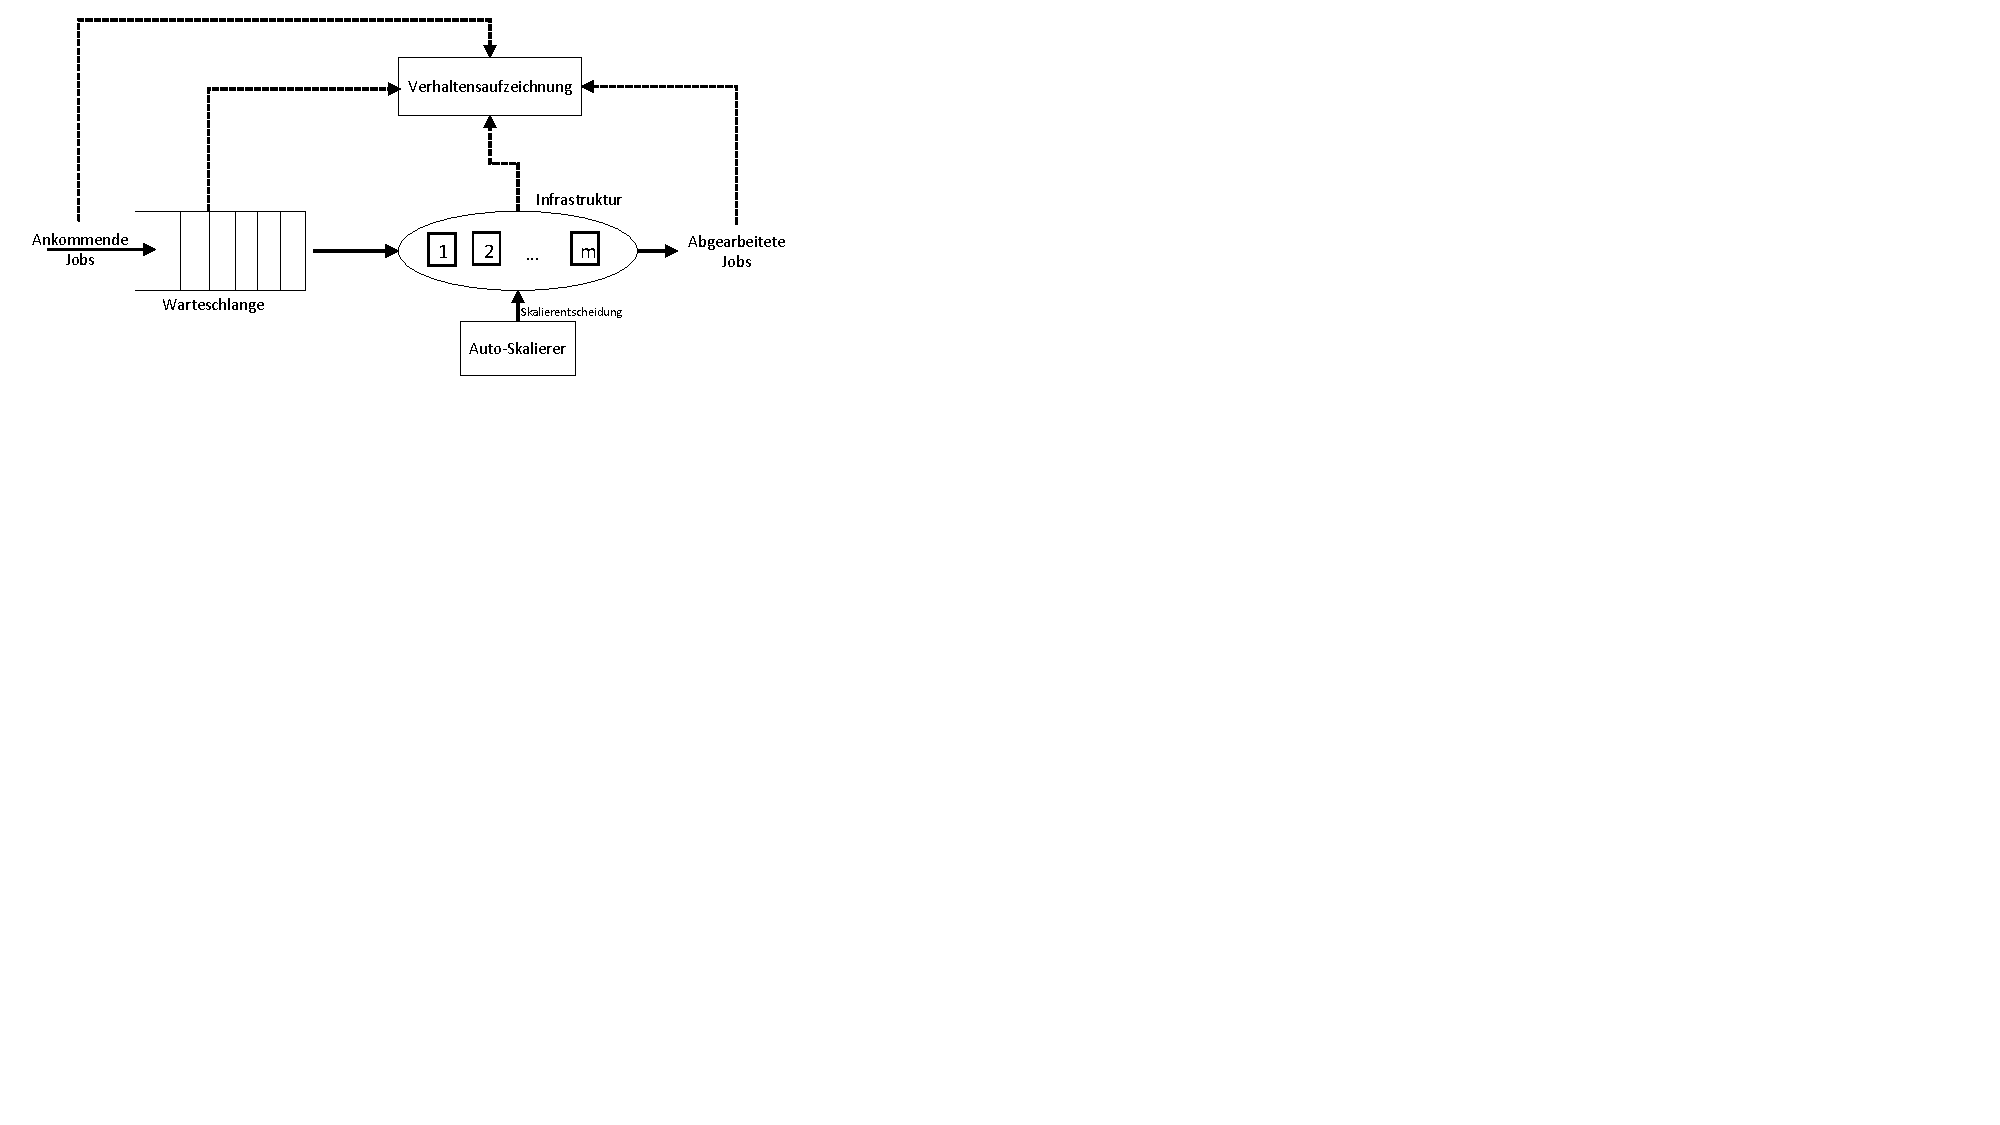
\includegraphics[width=\textwidth, trim={1cm 13cm 20cm 0cm}]{img/BasicIdea.pdf}
	\caption{Grundlegende Idee der Testbench}
	\label{fig:BasicIdea}
\end{figure}

\noindent
Zu einem Zeitpunkt \textit{t} erreicht eine (durch die gegebene Workload spezifizierte) Menge an Jobs das System und wird in der Warteschlange, die als Puffer fungiert, eingereiht. Die Infrastruktur wird durch eine Menge an Virtuellen Maschinen (\textit{VMs}) repräsentiert. Jede VM ist in der Lage in einer Zeiteinheit eine gewisse Menge an Jobs abzuarbeiten. Die Infrastruktur kann also pro Zeiteinheit eine durch die VMs definierte Menge an Jobs aus der Warteschlange nehmen und verarbeiten. Falls die Menge an ankommenden Jobs größer ist, als die Kapazität der Infrastruktur, so wird die Menge an wartenden Jobs in der Warteschlange größer. Diese Menge reduziert sich erst dann, wenn die Kapazität größer ist als die Last, wenn also entweder die Last unter dieses Level sinkt, oder aber die Kapazität durch eine Skalierentscheidung ausreichend vergrößert wird.\\
Allgemein ist die Testbench parametrisierbar. Beispielsweise soll die Warteschlangengröße und die Menge an maximal hinzuzufügenden VMs begrenzt sein. Weiterhin ist die Zeit zwischen Ankunft eines Jobs und dessen Abarbeitung in der Realität nicht gleich null. Diese und weitere Parameter können dynamisch konfiguriert werden, sodass nicht nur der Auto-Skalierer unter verschiedenen Lastbedingungen getestet werden kann, sondern auch auf unterschiedlich konfigurierten Infrastrukturen. \\
Um eine Skalier-Entscheidung treffen zu können, muss der Auto-Skalierer (je nach Typ) diverse Metriken der Infrastruktur oder der Warteschlange erheben, wie beispielsweise Länge der Warteschlange oder Auslastung der VMs. Dafür ist es notwendig, dass alle wichtigen Komponenten diese Metriken zu Verfügung stellen. \\
Um im Anschluss an eine Simulation den Auto-Skalierer bewerten zu können, wird der Zustand sämtlicher Komponenten zeitdiskret aufgezeichnet. Dabei werden Informationen wie Auslastung des Systems, Füllstand der Warteschlange, Durchsatz oder Wartezeiten im Puffer aufgezeichnet. Mittels dieser Daten kann dann das Verhalten des Auto-Skalierers, und damit seine Güte bestimmt werden.

\section{Übersicht}
\begin{itemize}
	\item \textbf{Kapitel \ref{ch:Architektur und Technologien}} beschreibt die verwendeten Technologien und die zugrundeliegende Architektur.
	
	\item In \textbf{Kapitel \ref{ch:Aufbau}} wird der Aufbau der Testbench auf Komponenten, bzw. Klassen-Ebene beschrieben. 
	\item Die Konfigurationsmöglichkeiten werden in \textbf{Kapitel \ref{ch:Konfiguration}} beschrieben.
	
	\item Abschließend wird die Applikation in \textbf{Kapitel \ref{ch:Evaluation} }evaluiert. Dafür werden Evaluationsaufbau- und Ergebnisse vorgestellt. Dieses Kapitel beendet die Dokumentation mit einer Zusammenfassung und einem Ausblick.
\end{itemize}

 




\chapter{Architektur und Technologien}
\label{ch:Architektur und Technologien}
Dieses Kapitel beschreibt die verwendeten Technologien und die Architektur der Testbench. Aufgabe ist es ein Kommandozeilen-basiertes Programm zu entwickeln, das basierend auf gegebenen Konfigurations-Dateien die Testbench startet und die Simulation durchführt. Die beobachteten Ergebnisse sollen anschließend wiederum in Dateien geschrieben werden



\section{Technologien}
\label{sec:Architektur und Technologien:Technologien}
Die vorgegebene, zu verwendende Programmiersprache ist Java. Weiterhin wird das Java-basierte Spring-Framework\footnote{https://spring.io/} verwendet, da es einige nützliche Features wie \textit{Dependency Injection} oder Event-basierte Kommunikation bietet. Als Applikationsserver wird durch Spring implizit eine leichtgewichtige Variante von Tomcat benutzt. Für den Augenblick besitzt der Auto-Skalierer keine Benutzeroberfläche und läuft auf einem lokalen Rechner. Mit Hinblick auf die Zukunft, könnte die Testbench entweder als Web-Applikation gestaltet werden, oder aber eine Benutzeroberfläche erhalten und als Desktop-Anwendung laufen. In beiden Fällen unterstützt das Spring-Framework diesen Evolutionsschritt enorm, sodass beide Varianten mit geringem Aufwand umgesetzt werden können. \\
Die Konfigurationen für die Testbench liegen im neutralen JSON-Format\footnote{https://www.json.org/} vor, da dieses sehr einfach eingelesen werden kann. Die Eingabe der Workload erfolgt ebenfalls im JSON-Format. \\
Die Ausgabe-Informationen sind zeit-diskrete, strukturierte Werte weshalb das Tabellen-Format \textit{CSV} zur Speicherung verwendet wird.


\section{Architektur}
\label{sec:Architektur und Technologien:Architektur}
Wie in Sektion \ref{fig:BasicIdea} beschrieben besteht die Testbench aus verschiedenen Modulen, die miteinander kommunizieren müssen. Gleichzeitig ist es wünschenswert, die Module lose zu koppeln und Austauschbar zu gestalten. Auch kann eine Informationsquelle bei der Testbench mehrere Informationssenken haben: Der Zustand der Infrastruktur muss periodisch an verschiedenste Komponenten gesendet werden wie zum Beispiel an die Module zur Aufzeichnung der diversen Metriken oder an den Auto-Skalierer. Weitere Informationssenken, die diese Information verarbeiten wollen, sollten dabei ohne größere Veränderung hinzugefügt werden können. Außerdem erzwingt die zeit-diskrete Simulation einen Taktgeber, der periodisch alle Komponenten über den nächsten Taktzyklus informiert. Direkte Kommunikation zwischen den jeweiligen Komponenten hätte dadurch einen nennenswerten Nachteil: Jede Komponente muss alle Komponenten kennen, mit denen sie kommunizieren muss. Im Falle des Taktgebers wären das sogar alle. \\
Event-basierte Architektur bietet einen Mechanismus, der das Versenden und Empfangen von Nachrichten entkoppelt. Damit ist es möglich die Module selbst zu entkoppeln und Nachrichtenaustausch über einen Event-Bus zu realisieren. Abbildung \ref{fig:EventBus} skizziert einen solchen Event Bus. Jede Komponente die eine Nachricht an andere Komponenten versenden möchte benötigt einen \textit{Event Publisher}, der eine (oder mehrere) Nachrichten versendet. Eine Nachricht hat dabei immer einen vordefinierten Typ. Jede Komponente die an dieser Nachricht interessiert ist, muss lediglich einen \textit{Event Listener} implementieren, der auf Nachrichten dieses Event-Typs hört. Falls eine weiteres Modul entwickelt wird, dass an bereits vorhandenen Nachrichtentypen interessiert ist (wie im Schaubild \textit{Event Listener 3}), so muss lediglich ein geeigneter Listener implementiert werden. Die anderen Module, vor allem die bereits implementierte Informationsquelle, muss fabei nicht verändert werden.  


%"l, b, r, t"
\begin{figure}[t]
	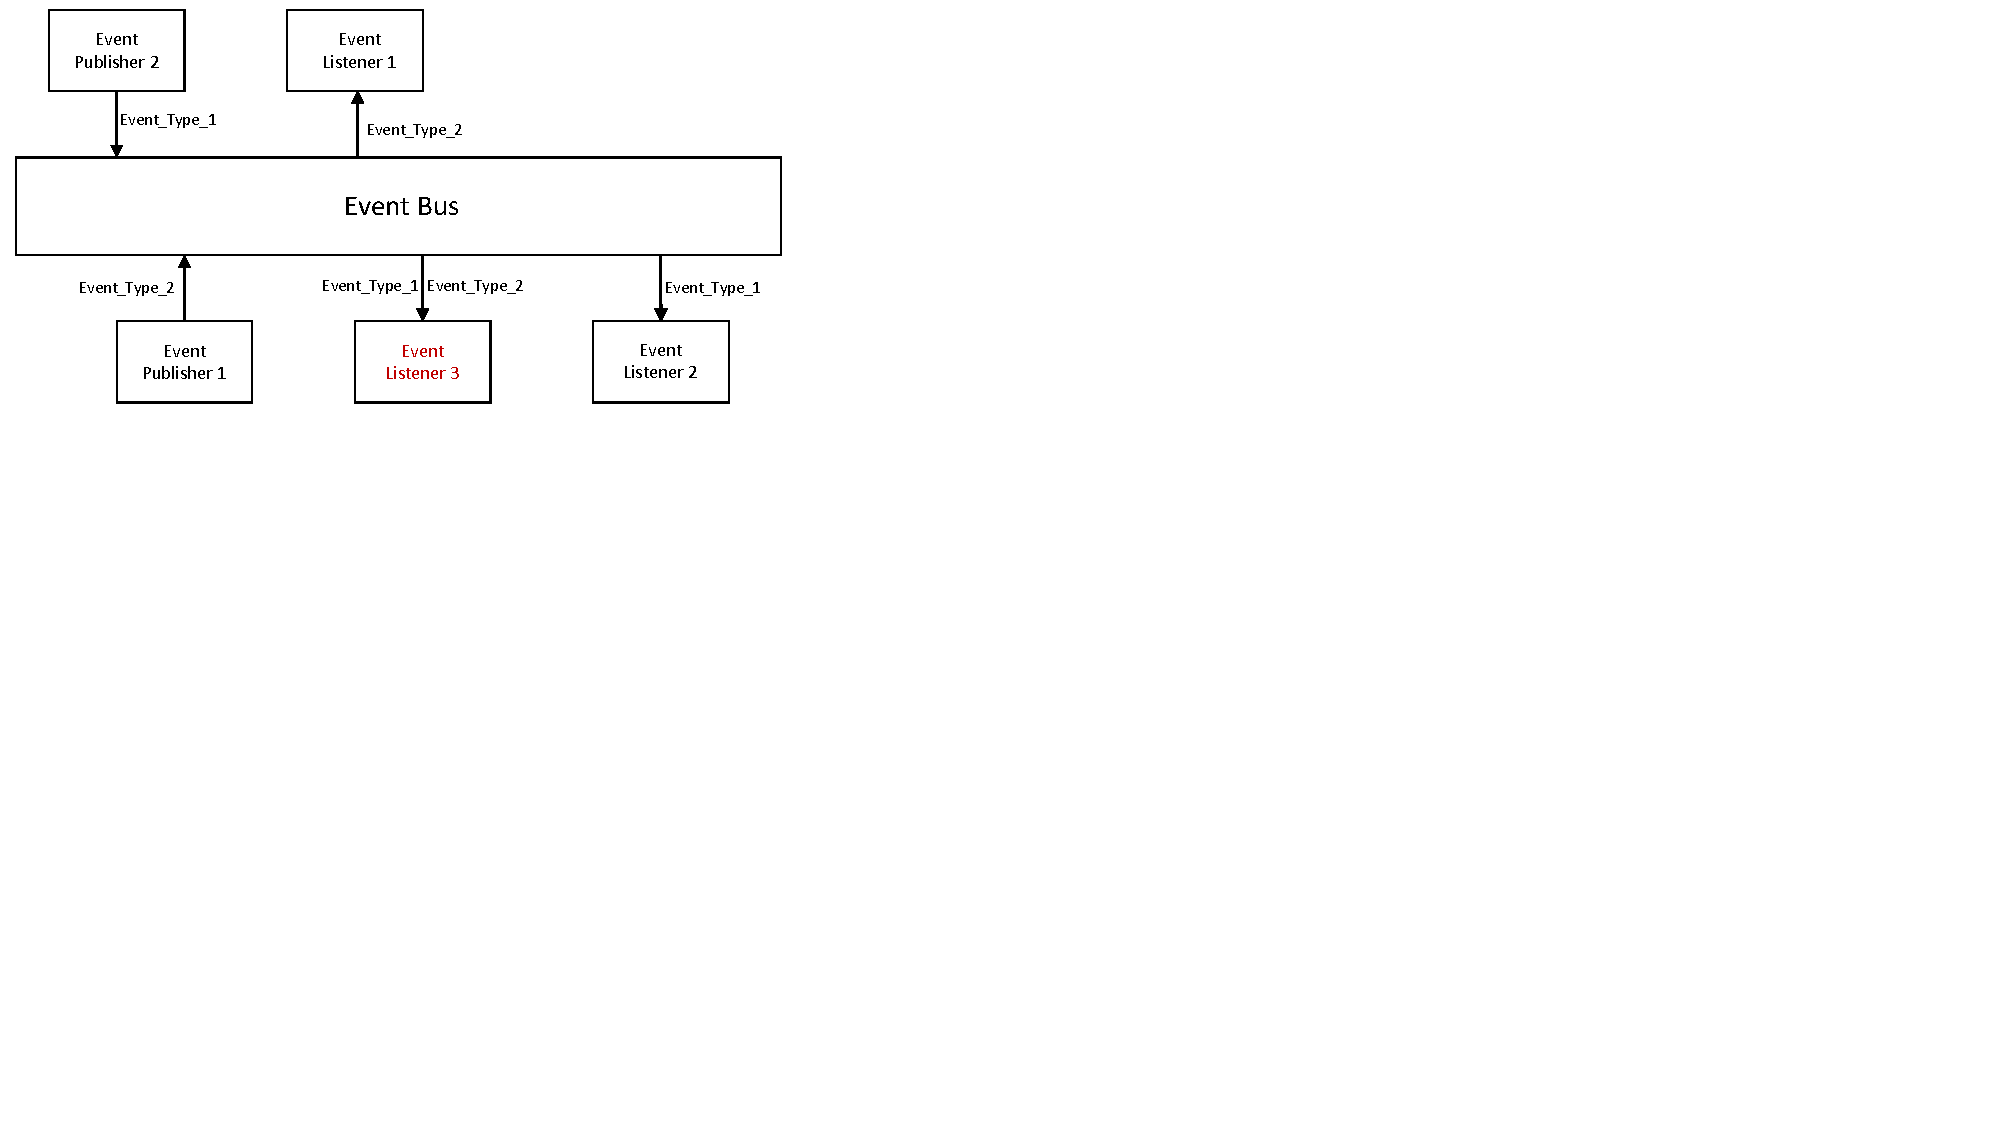
\includegraphics[width=\textwidth, trim={0cm 11.5cm 19cm 0cm}]{img/EventBus.pdf}
	\caption{Grundlegende Idee der Testbench}
	\label{fig:EventBus}
\end{figure}

\chapter{Aufbau}
\label{ch:Aufbau}
Dieses Kapitel beschreibt den konkreten Aufbau der Testbench. Wie in Sektion \ref{sec:Architektur und Technologien:Architektur} beschrieben, ist die verwendete Architektur Event-basiert. Abbildung \ref{fig:classDiagram} skizziert eine vereinfachte Form der Testbench in einer UML-Klassendiagramm ähnlichen Form. Aus Übersichtsgründen sind Utility-Klassen, Transfer-Objekte, POJO's\footnote{Plain Old Java Objects: Werden bspw. für die JSON-Deserialisierung benutzt} und die Event-Listener/Event-Publisher der Komponenten nicht Teil des Diagramms. Für jede Komponente, die eine Nachricht in Form eines Events an andere schicken oder von anderen empfangen möchte, existiert ein Listener beziehungsweise ein Publisher. Methoden des Listeners delegieren nach Empfang von Events die erhaltenen Nachrichten (Methodenaufrufe) an ihre nachgeschaltete Komponente. Komponenten die Nachrichten senden wollen, überreichen diese an ihren jeweiligen Publisher, der diese in Form eines Events auf den Event-Bus legt. Näheres ist in Sektion \ref{sec:Aufbau:Events} erklärt. \\
Im Folgenden werden alle wichtigen Systemkomponenten erläutert. Anschließend wird ein Überblick über die verschiedenen Event-Typen gegeben. Danach wir der zeitliche, sich periodisch wiederholende Ablauf eines Intervalls in der Testbench vorgestellt.









\section{Komponenten}
Abbildung \ref{fig:classDiagram} beschreibt den Zusammenhang aller Kern-Komponenten des Auto-Skalierers. Der Event-Bus selbst wird vom Spring-Framework bereitgestellt und ist nicht selbst implementiert. Die \textit{<<use>>} Bezeichnung soll lediglich verdeutlichen, dass die Komponenten Listener und/oder Publisher vorgeschaltet haben, die mit dem Event-Bus interagieren. Aus Gründen der Übersicht existieren keine Assoziations-Pfeile zwischen dem \textit{ApplicationStartUpRunner} und den Komponenten, die er initialisiert. Die Methodennamen lassen aber darauf schließen, mit welcher Komponente noch eine Assoziation existiert.

\subsection{Clock}
\label{sec:aufbau:Clock}
Die \textit{Clock} erfüllt die Aufgabe eines Taktgebers und ist somit das Herz der Testbench. In einer zeit-diskreten Simulation ist es solcher Taktgeber notwendig, da jede Komponenten über den Beginn eines neuen Intervalls informiert werden muss. Dabei gilt: Ein Intervall gilt erst dann als beendet, sobald jede Komponente ihre Aufgaben innerhalb dieses Intervalls erledigt hat. Nach Initialisierung der Komponenten arbeitet die Clock für eine in der Konfiguration definierte Anzahl an Intervallen (Simulationszeit). Dabei wird in jedem Schritt zuerst der Workload, falls notwendig, geändert. Danach versendet die Clock ein Event, dass den Beginn eines neuen Intervalls bekannt gibt. Alle Komponenten werden benachrichtigt und erledigen daraufhin ihre Arbeit, wie Verarbeitung der aktuell anliegenden Workload oder Ausführen von Skalier-Entscheidungen. Abschließend werden \textit{InfrastructureModel} und \textit{QueueModel} durch die Clock aufgefordert ihren aktuellen Zustand zu publizieren. Basierend darauf führen die Komponenten im nächsten Intervall ihre Aufgaben durch. 


\subsection{Infrastructure Model}
Das \textit{InfrastructureModel} bündelt die Haupt-Komponenten der Testbench. Es hat eine Warteschlange für ankommende und wartende Jobs (vgl.\ref{sec:aufbau:QueueModel}), eine Komponente die sich um das Hochfahren der Virtuellen Maschinen kümmert (vgl.\ref{sec:aufbau:BootinQueu}) sowie einen gekapselten Zustand (vgl.\ref{sec:aufbau:State}). \\
Die Information, wie viel Last in welchem Zeitintervall anliegt, wird im \textit{InfrastructureModel} gespeichert und ggf. durch Erhalt einer Workload-Änderung (\textit{changeWorkload()}) geändert. Basierend darauf, ist sie verantwortlich bei Erhalt eines jeden Clock-Ticks (\textit{handleClockTick()}) die erforderliche Menge an Jobs in der Warteschlange (vgl.\ref{sec:aufbau:QueueModel}) einzureihen. Danach berechnet das \textit{InfrastructureModel} als Abstraktion der Infrastruktur die vorhandene Kapazität an Jobs, die in diesem Intervall abgearbeitet werden können (abhängig von Anzahl der vorhandenen Virtuellem Maschinen) und nimmt diese Anzahl aus der Warteschlange und verarbeitet sie. \\
Unregelmäßig muss das Model mit Skalier-Entscheidungen des Auto-Skalieres umgehen (\textit{scaleVirtualMachines()}). Dabei werden hochfahrende Virtuelle Maschinen in der \textit{VMBootingQueue} eingereiht und nach abgelaufener Boot-Zeit mit in die Kapazitäts-Berechnung eingenommen. Das herunterfahren ist einfachheitshalber instantan.\\
Zuletzt kann der Zustand \textit{(vgl.\ref{sec:aufbau:State})} über die Methode \textit{publishInfrastructureState()} publiziert werden. Dieser Vorgang wird wie in Sektion\ref{sec:aufbau:Clock} beschrieben, von \textit{Clock} angestoßen.

\subsubsection{VM Booting Queue}
\label{sec:aufbau:BootinQueu}
Diese Komponente ist eine Warteschlange für hochzufahrende VMs. Nach dem Erhalt einer Skalier-Entscheidung (Hinzufügen einer VM), darf das \textit{InfrastructureModel} diese nicht direkt umsetzen, da eine VM eine gewisse Zeit braucht, um hochzufahren bevor sie aktiv mit in die Kapazitätsberechnung. Deswegen wird eine VM mittels \textit{addVirtualMachineToQueue()} hinzugefügt. In jedem Zeitintervall wird die zu wartende Zeit reduziert und überprüft, ob eine VM bereit ist und zur Menge der aktiv arbeitenden hinzugefügt werden kann \textit{(selectAndRemoveBootedVM())}.  


\subsection{Infrastructure State}
\label{sec:aufbau:State}
Der Zustand der Infrastruktur ist von der Funktionalität abgekapselt. Dieser speichert die aktuell anliegende Workload\textit{(currentArrivalRate)} sowie die aktiven VMs und damit die Kapazität. Der Zustand kann in ein \textit{TransferObject} verpackt und versendet werden. Dieses Objekt beinhaltet zusätzlich Informationen übe die CPU-Auslastung (Diskrepanz zwischen Kapazität und Anzahl der Tasks, die in einem Intervall das System verlassen).

%"l, b, r, t"
\begin{figure}[!h]
	\centering
	\begin{sideways}
		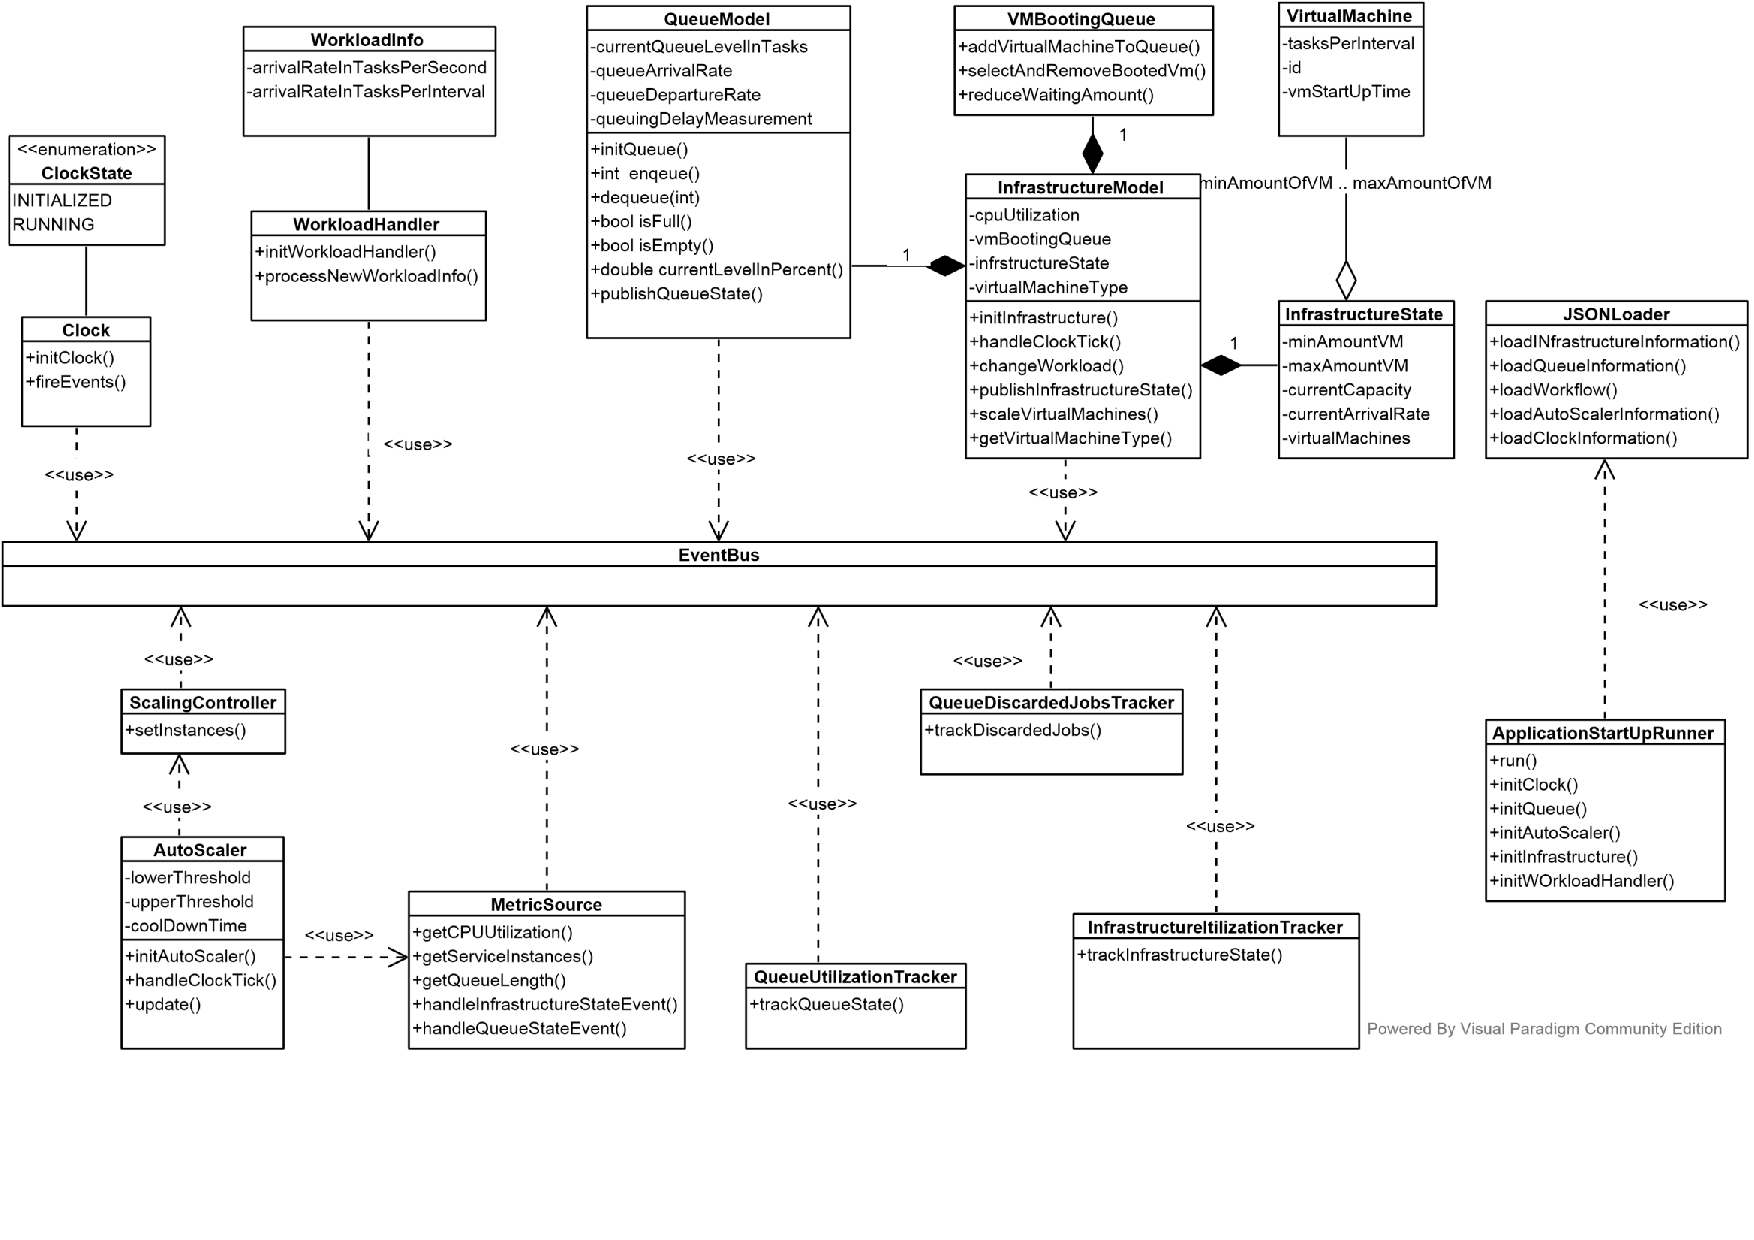
\includegraphics[width=20.0cm, trim={0cm 0cm 0cm 0cm}]{img/classDiagram.pdf}
	\end{sideways}
	\caption{Aufbau des Auto-Skalierers}
	\label{fig:classDiagram}
\end{figure}

\newpage

\subsection{Virtual Machine}
\label{sec:aufbau:VM}
Eine Virtuelle Maschine ist eindeutig durch ihre Id identifizierbar. Jede VM benötigt eine vordefinierte Zeit zum hochfahren \textit{vmStartUpTime} und kann pro Zeitintervall eine gewisse Anzahl an Jobs verarbeiten\textit{tasksPerInterval}. Die beiden letzten Werte sind bei dieser Testbench für alle Maschinen pro Simulation gleich, werden also einmalig bei Simulationsstart als Konfigurationsparameter mitgegeben.





\subsection{Auto Scaler}
Der \textit{AutoScaler} als solcher ist kein Teil der Testbench, da er ja das Testobjekt ist. In diesem Fall ist er lediglich hinzugefügt, um die Funktionalität der Testbench zu testen. Ein Auto-Scaler wird angebunden, indem er System-Metriken wie Auslastung oder Warteschlangenlänge über die Komponente \textit{MetricSource} bezieht und Skalierentscheidungen an die Komponente \textit{ScalingController} weiterreicht. Die Interfaces zur Anbindung eines Auto-Skalierers sind in Sektion\ref{sec:Konfiguration:AnbindungScaler} beschrieben.



\subsubsection{Scaling Controller}
Der \textit{ScalingController} bietet lediglich eine Schnittstelle für einen Auto-Skalierer, um Skalier-Entscheidungen an die Infrastruktur zu propagieren. Dabei wird der \textit{ScalingMode} zusammen mit den VMs, die entweder hoch- oder heruntergefahren werden sollen, übergeben.


\subsubsection{Metric Source}
Die \textit{MetricSource} bietet eine Schnittstelle für den Auto-Skalierer, um Metriken der Infrastruktur, wie bspw. die CPU-Auslastung oder die Warteschlangenlänge abzugreifen. Diese Metriken liegen immer als moving average vor, wobei das Fenster in den Konfiguration festgelegt werden kann.



\subsection{Queue Model}
\label{sec:aufbau:QueueModel}
Die Warteschlange definiert zwei grundlegende Aufgabe: Zuerst werden alle ankommenden Jobs in der Warteschlange eingereiht. Auch dann, wenn die Infrastruktur nicht völlig ausgelastet ist. Dies liegt an der Natur einer Cloud-Infrastruktur: Ein Job kann nicht in null Zeit ankommen und verarbeitet werden. Diese Verarbeitungszeit wird mit einer Warteschlange simuliert, die als FIFO-Liste aufgebaut ist. Ankommende Jobs können die Warteschlange erst verlassen, wenn sie mindestens für die Warteschlangenverzögerung \textit{(queuing delay)}. \\
Des Weiteren verhält sich die Warteschlange als Pufferspeicher: Falls die anliegende Last auf dem System größer als dessen Kapazität ist füllt sie sich. Ist es umgekehrt, so leert sie sich wieder. Da Puffer-Speicher in der Realität nicht unendlich groß sind, hat die Warteschlange eine Maximalkapazität. Ist diese erreicht, so werden weitere Jobs verworfen. \\
Wie auch das \textit{InfrastructureModel} muss die Warteschlange nach einer vordefinierten Zeit ihren Zustand publizieren, sodass \textit{Tracker} und die \textit{MetricSource} diesen auslesen können.

\subsection{Workload Handler}
Der \textit{WorkloadHandler} verarbeitet die zu simulierende Last auf dem System. Diese ist eine Eingabe als Liste von Werten. Der \textit{WorkloadHandler} verarbeitet nach einer frei konfigurierbaren Zeit den nächsten Eintrag und informiert das \textit{InfrastructureModel}, dass sie die Last geändert hat. Damit wird umgangen, dass tatsächlich Last generiert werden muss. Die Infrastruktur bekommt lediglich Informationen darüber, zu welchem Zeitpunkt wie viel Last anliegt. 

\subsubsection{Workload Info}
\textit{WorkloadInfo} ist eine Klasse, die eine Last zu einem bestimmten Zeitpunkt beschreibt.

\subsection{Tracker}
Die verschiedenen \textit{Tracker} zeichnen die Simulation zeit-diskret auf. Die Informationen können anschließend benutzt werden, um den Auto-Skalierer zu beurteilen. Alle aufgezeichneten Parameter werden durch Aufzeichnung der Zustände der jeweiligen Komponenten erhoben. Dabei wird ein gleitender Mittelwert bestimmt, um glattere Ergebnisse zu bekommen.

\subsubsection{Queue Utilization Tracker}
Dieser \textit{Tracker} zeichnet folgende Parameter auf:
\begin{itemize}
	\item Anzahl an wartenden Jobs 
	\item Füllstand in Prozent, gemessen an der maximalen Länge
	\item Ankunftsrate
	\item Verarbeitungsrate (Menge an Jobs, die die  Warteschlange verlassen)
	\item Durchschnittliche Wartezeit in der Warteschlange
\end{itemize}

\subsubsection{Queue Discarded Jobs Tracker}
Dieser \textit{Tracker} zeichnet folgende Parameter auf:
\begin{itemize}
	\item Anzahl an verworfenen Jobs Pro Intervall
\end{itemize}

\subsubsection{Infrastructure Utilization Tracker}
\begin{itemize}
	\item Ankunftsrate
	\item Verarbeitungsrate (Menge an Jobs, die das System verlassen)
	\item Kapazität (Menge an Jobs, die alle VMs verarbeiten können)
	\item Anzahl der Virtuellen Maschinen
	\item CPU Auslastung
\end{itemize}

\subsection{Application Start Up Runner}
Diese Komponente liest die Konfigurationen via \textit{JSONLoader} und initialisiert alle anderen Komponenten. Dies beinhaltet die Umrechnung der externen Einheit (Parameter gegeben in Millisekunden) in die interne Einheit (gegeben in Clock-Ticks). Anschließend startet sie die Simulation.

\subsection{JSON Loader}
Der \textit{JSONLoader} ist eine Klasse zum laden und serialisieren der Konfigurationen im JSON-Format. Jede Konfigurations-Datei wird dabei mittels \textit{Object-Mapper} auf eine Klasse abgebildet.

\section{Events}
\label{sec:Aufbau:Events}
Für die Kommunikation zwischen den Komponenten, beziehungsweise um das Auslösen einer Handlung (Methodenaufruf) einer speziellen Komponente anzustoßen, werden Events benutzt. Abbildung \ref{fig:eventsDiagram} zeigt, dass alle Events von einem \textit{AbstractEvent} erben, in dem der aktuelle Clock-Zähler und die feste Intervall-Dauer gegeben ist. Diese Informationen sind somit in jedem Event verfügbar, sodass man das Event einem diskreten Zeitintervall zuordnen kann. Im folgenden wird darauf eingegangen, was ein Event absetzt und für was es bestimmt ist.



\begin{itemize}


	\item \textit{FinishSimulationEvent} 
	\begin{itemize}
         \item \textbf{Absender:} \textit{Clock}
         \item \textbf{Empfänger:} Alle Tracker
         \item \textbf{Grund:} Erstellen der Ausgabedateien, Schließen der File-Writer
         \item \textbf{Parameter:} Skalierfaktor, zurückrechnen in Ausgabeformat
 	\end{itemize} 
     
    	\item \textit{StartSimulationEvent} 
    \begin{itemize}
    	\item \textbf{Absender:} \textit{Clock}
    	\item \textbf{Empfänger:} Alle Tracker
    	\item \textbf{Grund:} Beenden des Schreibens in die jeweiligen Dateien
    \end{itemize} 

	\item \textit{ClockEvent} 
\begin{itemize}
	\item \textbf{Absender:} \textit{Clock}
	\item \textbf{Empfänger:} \textit{InfrastructureModel}, \textit{AutoScaler}
	\item \textbf{Grund:} Beginn neues Intervall
\end{itemize} 

	\item \textit{TriggerPublishInfrastructureStateEvent} 
\begin{itemize}
	\item \textbf{Absender:} \textit{Clock}
	\item \textbf{Empfänger:}  \textit{InfrastructureModel}
	\item \textbf{Grund:} Infrastruktur soll Zustand publizieren
\end{itemize} 

	\item \textit{TriggerPublishQueueStateEvent} 
\begin{itemize}
	\item \textbf{Absender:} \textit{Clock}
	\item \textbf{Empfänger:} \textit{QueueModel}
	\item \textbf{Grund:} Warteschlange soll Zustand publizieren
\end{itemize} 

	\item \textit{TriggerWorkloadHandlerEvent} 
\begin{itemize}
	\item \textbf{Absender:} \textit{Clock}
	\item \textbf{Empfänger:} \textit{WorkloadHandler}
	\item \textbf{Grund:} Neue Workload publizieren
\end{itemize} 

	\item \textit{ScalingEvent} 
\begin{itemize}
	\item \textbf{Absender:} \textit{ScalingController}
	\item \textbf{Empfänger:} \textit{InfrastructureModel}
	\item \textbf{Grund:} Neue Skalier-Entscheidung getroffen
	\item \textbf{Parameter:} Skalier-Modus und jeweilige VM-Instanzen
\end{itemize} 

	\item \textit{QueueStateEvent} 
\begin{itemize}
	\item \textbf{Absender:} \textit{QueueModel}
	\item \textbf{Empfänger:} \textit{QueueTracker}
	\item \textbf{Grund:} Zustand der Warteschlange soll geschrieben werden
	\item \textbf{Parameter:} Enthält Infos über Zustand, die in Datei geschrieben werden sollen
\end{itemize} 



	\item \textit{WorkloadChangedEvent} 
\begin{itemize}
	\item \textbf{Absender:} \textit{WorkloadHandler}
	\item \textbf{Empfänger:} \textit{InfrastructureModel}
	\item \textbf{Grund:} Veränderung der Workload
	\item \textbf{Parameter:} Neue Workload
\end{itemize} 

	\item \textit{DiscardedJobsEvent} 
\begin{itemize}
	\item \textbf{Absender:} \textit{QueueModel}
	\item \textbf{Empfänger:} \textit{QueueTracker}
	\item \textbf{Grund:} Jobs wurden verworfen, da Warteschlange übergelaufen ist
	\item \textbf{Parameter:} Anzahl der verworfenen Jobs im Zeitintervall
\end{itemize} 

	\item \textit{InfrastructureStateEvent} 
\begin{itemize}
	\item \textbf{Absender:} \textit{InfrastructureModel}
	\item \textbf{Empfänger:} \textit{InfrastructureTracker}
	\item \textbf{Grund:}  Zustand der Infrastruktur soll geschrieben werden
	\item \textbf{Parameter:} Enthält Infos über Zustand, die in Datei geschrieben werden sollen
\end{itemize} 





\end{itemize}
 

%"l, b, r, t"
\begin{figure}[!h]
	\centering
	
	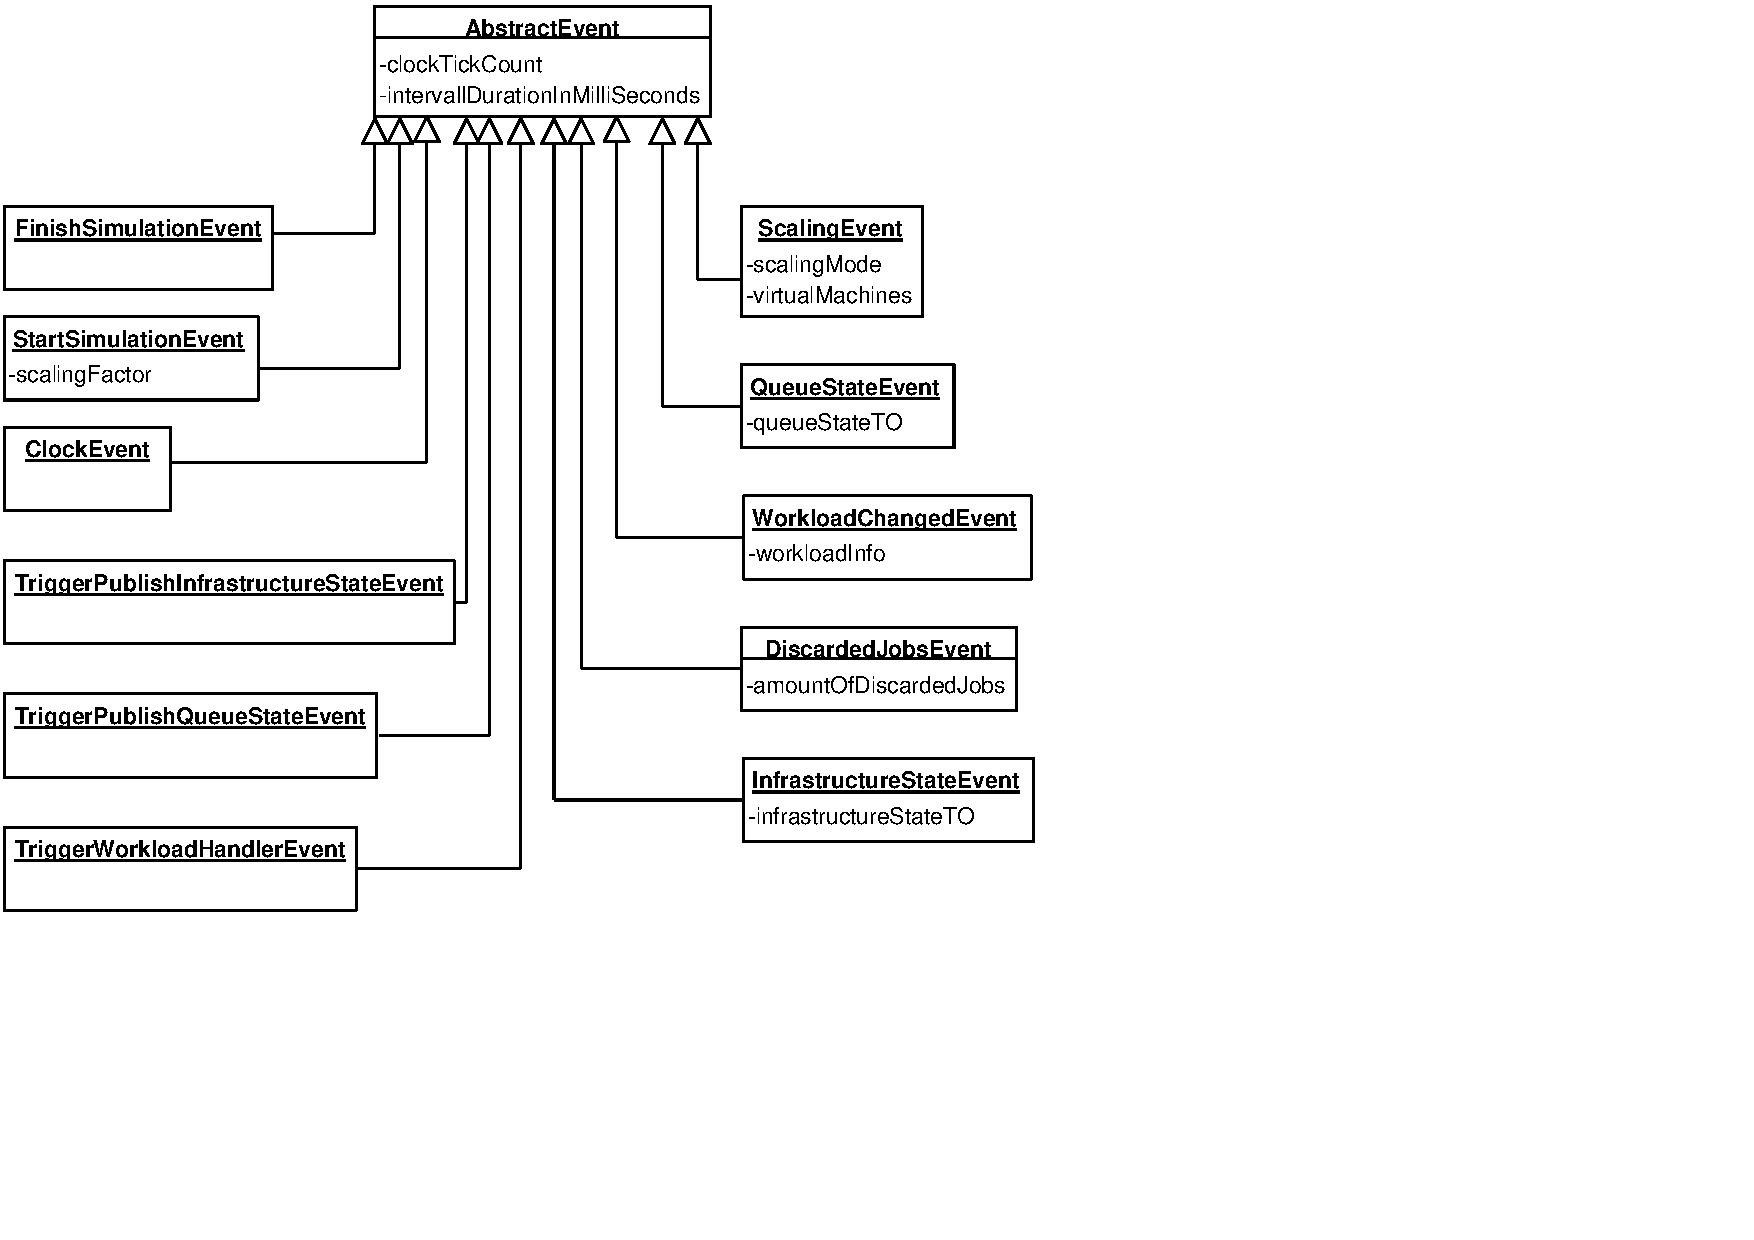
\includegraphics[width=20.0cm, trim={0cm 5cm 6cm 0cm}]{img/eventsDiagram.pdf}
	
	\caption{Übersicht der Events}
	\label{fig:eventsDiagram}
\end{figure}


gtrge

\section{Ablauf}

gerger


\chapter{Konfiguration}
\label{ch:Konfiguration}
Während Kapitel \ref{ch:Aufbau} den Aufbau der Testbench beschreibt, befasst sich dieses mit deren Konfiguration. Da sie so flexibel wie möglich gehalten ist, muss der Benutzer Komponenten wie die Infrastruktur, die Warteschlange, Virtuelle Maschinen und die Auflösung der zeit-diskreten Simulation parametrisieren. Die verwendeten Parameter sollten möglichst nahe der Realität entsprechen, sodass die Simulationsergebnisse korrekt sind. Im folgenden werden die einzelnen Konfigurationsdateien beschreiben, sowie die Anbindung eines individuellen Auto-Skalierers und ein weiterer Tracker.

\section{Einheiten}
Die externe Einheit der zeit-diskreten Simulation wird in Millisekunden angegeben. Intern werden diese in Clock-Ticks umgerechnet. So wird etwa die benötigte Zeit zum Hochfahren einer Virtuellen Maschine (in [ms]) umgerechnet in die Anzahl an Clock-Ticks. Dies ist notwendig, da der Benutzer die Konfigurationsparameter in Millisekunden (oder einer Potenz davon) vorliegen hat. Abhängig von der Auflösung eine Zeitintervalls, also Abstand zwischen zwei Clock-Ticks, wird dieser Wert in Clock-Ticks umgerechnet.


\section{Konfigurationsparameter}
Fünf verschiedene Konfigurationsdateien liegen vor. Diese befinden sich im Verzeichnis \\ \textit{src/main/data}. Für die Zukunft ist geplant, den Pfad dieser Dateien über die Kommandozeile beim Ausführen der Applikation zu übergeben.

\subsection{Clock}
\label{sec:konfiguration:clock}
Die Datei \textit{clock.json} beschreibt die grundlegenden Parameter für die Auflösung der Simulation und die Zeitintervalle, in denen diverse Komponenten angestoßen werden. 

\begin{lstlisting}[language=json,firstnumber=1, caption={clock.json}]
{
  "millisecondsTillPublishInfrastructureState": 500,
  "millisecondsTillPublishQueueState": 500,
  "intervalDurationInMilliSeconds": 100,
  "millisecondsTillWorkloadChange": 1000,
  "experimentDurationInMinutes": 7 
}
\end{lstlisting}

\begin{itemize}
	\item \textbf{Zeile 2:} Alle 500ms soll die Infrastruktur ihren Zustand publizieren
	\item \textbf{Zeile 3:} Alle 500ms soll die Warteschlange ihren Zustand publizieren
	\item \textbf{Zeile 4:} Intervallbreite, Die Zeit zwischen zwei Clock-Ticks soll 100ms betragen 
	\item \textbf{Zeile 5:} Jede Sekunde soll sich die Workload ändern
	\item \textbf{Zeile 6:} Die Simulationszeit soll sieben Minuten betragen
	
\end{itemize}
\noindent
Es ist zu beachten, dass alle Werte (außer die Simulationsdauer) ein Vielfaches der Intervallbreite sind. Ist dies nicht der Fall, kommt es ggf. zu Rundungsfehler, die die Simulationsergebnisse verfälschen. \\
 \textbf{Beispiel:} Intervallbreite = 100ms; Workload-Änderung alle 1000ms. Daraus folgt, dass die Workload alle 10 Clock-Ticks geändert wird. Wird beispielsweise die Workload-Änderung mit 1049ms angegeben, so wird sie immer noch mit 10 Clock-Ticks umgerechnet (durch interne Rundung).
 


\subsection{Infrastruktur}
\label{sec:konfiguration:infrastruktur}
Die Datei \textit{infrastructure.json} parametrisiert das \textit{InfrastructureModel}. Die Infrastruktur soll immer nur einen VM-Typ zulassen. 
\begin{lstlisting}[language=json,firstnumber=1, caption={infrastructure.json}]
{
  "virtualMachineType": 
    {
     "millisecondsPerTask": 500,
     "vmStartUpTimeInMilliSeconds": 3000
    },
  "amountOfVmsAtSimulationStart": 1,
  "cpuUitilizationWindow" : 20
}
\end{lstlisting}


\begin{itemize}
	\item \textbf{Zeile 2-6:} Beschreibung des VM-Typs; jede VM benötigt 500ms um einen Job abzuarbeiten. Die Zeit zum hochfahren beträgt 3000ms
	\item \textbf{Zeile 7:} Zu Beginn soll eine VM gestartet sein
	\item \textbf{Zeile 8:} Anzahl der Intervalle, über die ein gleitender Mittelwert der CPU-Auslastung gemessen wird  
	
\end{itemize}
Durch einen internen Skalierfaktor ist es möglich, dass die Abarbeitung eines Tasks über mehrere Intervallgrenzen hinausgeht. Das CPU-Fenster sollte in Relation zu der Intervallbreite und dem Abstand, mit dem der Zustand der Infrastruktur publiziert wird gesetzt werden (beide Werte in \textit{clock.json} definiert). \\
\textbf{Beispiel:} Aus \textit{clock.json} geht hervor, dass alle 10 Clock-Ticks der Zustand der Infrastruktur zu publizieren ist. Deshalb sollte der angegebene Wert größer als 10 sein, damit alle Clock-Ticks seit der letzten Publizierung in die Berechnung mit einfließen. Ein Wert von 20 bedeutet somit, dass der Mittelwert der letzten Zustandspublikationen noch mit einfließt.


\subsection{AutoScaler}
Die Datei \textit{autoscaler.json} beschreibt das Verhalten des implementierten Auto-Skalierers. Falls ein anderer implementiert und angebunden wird, so muss auch diese Datei angepasst werden. Eventuell kommen hier weitere Felder hinzu, da ein anderer Scaler andere Konfigurationsparameter erwartet. Diese hier gelten nur für den verwendeten Prototyp.








\begin{lstlisting}[language=json,firstnumber=1, caption={autoscaler.json}]
{
  "lowerThreshold": 0.25,
  "upperThreshold": 0.75,
  "vmMax": 20,
  "vmMin": 1,
  "timeInMsTillNextScalingDecision": 1000,
  "cpuUtilWindow" : 10,
  "queueLengthWindow": 10,
  "coolDownTimeInMilliSeconds": 100000
}
\end{lstlisting}

\begin{itemize}
	\item \textbf{Zeile 2:} Auslastung, ab die der Scaler runter skalieren soll (25\%)
	\item \textbf{Zeile 3:} Auslastung, ab die der Scaler hoch skalieren soll (75\%)
	\item \textbf{Zeile 4:} Maximale Anzahl Virtueller Maschinen; Ist diese erreicht, so wird auch bei einer Auslastung >75\% nicht weiter hoch skaliert
	\item \textbf{Zeile 5:} Minimale Anzahl Virtueller Maschinen; verhält sich invers zu Zeile 4
	\item \textbf{Zeile 6:} Zeit zwischen zwei aufeinanderfolgenden Skalier-Entscheidungen
	\item \textbf{Zeile 7:} Anzahl der zu betrachteten Status-Updates der CPU-Auslastung für einen gleitenden Mittelwert
	\item \textbf{Zeile 8:} Wie Z.7, nur für die Queue-Länge 
	\item \textbf{Zeile 9:} Zeit nach einer ausgeführten Skalier-Entscheidung, in der der Scaler nichts ausführen soll 
	
\end{itemize}

\noindent
Zeile 7 und Zeile 8 sind Parameter, die für die \textit{MetricSource} zu Verfügung gestellt werden müssen. Diese müssen also auch bei einem anderen Scaler in der Konfigurationsdatei definiert sein. Auch hier ist zu beachten, dass der Parameter in Zeile 6 ein Vielfaches der Intervallbreite aus \textit{clock.json} ist.

\subsection{Queue}
Die Datei \textit{queue.json} beschreibt die Konfigurationsparameter für die Warteschlange.



\begin{lstlisting}[language=json,firstnumber=1, caption={queue.json}]
{
  "queueLengthMax": 80000,
  "windowSize" : 20,
  "queuingDelayInMilliSeconds": 100
} 
\end{lstlisting}

\begin{itemize}
	\item \textbf{Zeile 2:} Maximale Anzahl an Jobs, die in die Warteschlange passen. Ist diese erreicht, so werden weitere Jobs verworfen.
	\item \textbf{Zeile 3:} Anzahl der Intervalle, über die ein gleitender Mittelwert der Warteschlangen-Länge gemessen wird  
	\item \textbf{Zeile 4:} Warteschlangenverzögerung, Zeit die ein Jobs braucht zwischen Ankunft im System und verlassen der Warteschlange, bzw. Abarbeitung im System
	
\end{itemize}

Die Fenstergröße sollte analog wie die Fenstergröße in Sektion \ref{sec:konfiguration:infrastruktur} gewählt werden. Außerdem ist zu beachten, dass die Verzögerungszeit ebenfalls als Vielfaches der Auflösung zu wählen ist.

\subsection{Workflow}
Die Datei \textit{workflow.json} beschreibt den Workflow, also die Last die am System zu einem Zeitpunkt anliegen soll. Dabei entspricht jeder Wert der Anzahl an Jobs, die zwischen zwei Workload-Änderungen abzuarbeiten ist. Intern wird dieser Wert also wie folgt umgerechnet:\\
Gegeben sei der erste Wert (=7) aus der Liste. Aus \textit{clock.json} geht hervor, dass eine Workload-Änderung alle 1000ms passiert. In dieser Zeit sollen also sieben Jobs abgearbeitet werden. Da die Intervallbreite 100ms beträgt, errechnet sich der Wert $\dfrac{7 Jobs * 100ms}{1000ms * Interval}$ = $\dfrac{0.7Jobs}{Interval}$. \\

\vspace{0.2cm}
\noindent
Aus diesem Grund wird intern skaliert, sodass auch mit solch "kleinen" Werten umgegangen werden kann.


\begin{lstlisting}[language=json,firstnumber=1, caption={workflow.json}]
{
  "workflow": [
    7.0,
    5.0,
    8.0,
    6.0,
   ]
}
\end{lstlisting}




\section{Anbindung eines Auto-Skalierers}
\label{sec:Konfiguration:AnbindungScaler}
Um einen eigenen Auto-Skalierer zu implementieren, muss eine Klasse erstellt werden, die das Interface \textit{IAutoScaler} in Abbildung \ref{lst:scaler} implementiert. Ein Beispiel dafür ist die Abbildung \ref{lst:customScaler}. \\
Zuerst muss die bestehende Implementierung entweder gelöscht werden, oder deren Bezeichner im \textit{@Component-Tag} geändert werden. Das Framework benutzt immer den Skalierer mit dem eindeutig vergebenen Namen \textit{@Component(''activeScaler")}. \\
Falls andere Konfigurationsparameter benutzt werden müssen, wie die die in \textit{initAutoScaler()} definiert sind, so muss eine gröberer Änderung vorgenommen werden, die hier nur oberflächlich skizziert wird:
\begin{itemize}
	\item Ergänze/Lösche Parameter in \textit{autoscaler.json}
	\item Analog dazu Felder+Getter*Setter in \textit{AutoScalerPOJO.java}
	\item Adaptiere \textit{initAutoScaler()} in \textit{IAutoScaler.java} und der eigenen Implementierung
	\item Instanziiere der AutoScaler mit den korrekten Attributen in \textit{ApplicationStartUpRunner.java}, Methode \textit{initAutoScalerAndMetricSource()}.
\end{itemize}

\noindent
Die eigene Implementierung muss die Logik komplett selbst implementieren. Das bedeutet, \textit{handleClockTick()} wird in jedem Intervall vom Taktgeber der Infrastruktur angestoßen. Der Auto-Skalierer ist selbst dafür verantwortlich, wann er welche Skalier-Entscheidung trifft, auf welchen Metriken er diese begründet, wie viele VMs hoch-oder heruntergefahren werden oder wie lange seine CoolDown-Phase ist. Dafür stehen die beiden Schnittstellen \textit{IMetricSource} (Abbildung \ref{lst:metric}) und \textit{IScalingController} (Abbildung \ref{lst:controller}) zu Verfügung. \\
Die \textit{IMetricSource} stellt eine Schnittstelle zum Abrufen von Metriken da. Außerdem kann darüber abgerufen werden, welche VMs gerade aktiv sind. Dies ist notwendig, denn bei einer Skalier-Entscheidung (Modus \textit{'SCALE\_DOWN'} aus Abbildung \ref{lst:mode}), muss dem \textit{IScalingController} (Abbildung \ref{lst:controller})eine Liste der VMs übergeben werden, die herunterzufahren sind. Identifiziert werden diese über eine eindeutig vergebene ID. Sollten neue VMs hochgefahren werden, müssen diese mit den Parameter, die über die Methode \textit{getVirtualMachineType()} ausgelesen werden können und einer eindeutigen ID (ggf. UUID), erzeugt werden. \\

\begin{lstlisting}[language=Java,firstnumber=1, caption={CustomScaler.java}, label=lst:customScaler]
@Component("activeScaler")
public class CustomScaler implements IAutoScaler{
  
  @Autowired
  private IScalingController scalingController;
  
  @Autowired
  private IMetricSource metricSource;
  
  @Override
  public void initAutoScaler(double lowerThreshold, double upperThreshold, int vmMin, int vmMax,
    int coolDownTimeInIntervallTicks, int clockTicksTillScalingDecision) {
    // implement logic here
  }

  @Override
  public void handleClockTick(ClockEvent event) {
    // implement logic here
  }
}
\end{lstlisting}




\begin{lstlisting}[language=Java,firstnumber=1, caption={IAutoScaler.java}, label=lst:scaler]
public interface IAutoScaler {

  /**
  * AutoScaler is initialized with those parameters
  */
  void initAutoScaler(double lowerThreshold, double upperThreshold, int vmMin, int vmMax,
       int coolDownTimeInIntervallTicks, int clockTicksTillScalingDecision);

  /**
  * Implement Logic. Proactive scaling decision! Need to check each clockTick if
  * scaling decision needs to be executed.
  * This includes to administer coolDown counter.
  * 
  * @param event
  */
  void handleClockTick(ClockEvent event);

}
\end{lstlisting}


\begin{lstlisting}[language=Java,firstnumber=1, caption={IMetricSource.java}, label=lst:metric]
public interface IMetricSource {

  /**
  * Moving Average of CPU-Utilization
  */
  public double getCPUUtilization();

  /**
  * Moving Average of Queue-Length
  */
  public int getQueueLength();

  /**
  * Retrieve currently available List of active Virtual Machines
  */
  public List<VirtualMachine> getServiceInstances();

  /**
  * Return Infrastructure-State at a certain Clock-Interval
  */
  public InfrastructureStateTransferObject getInfrastructureState();


  /**
  * Information of currently used VM-Type! For a Scaling decision, it is needed
  * to instantiate VMs with those parameters
  */
  public VirtualMachineType getVirtualMachineType();
}
\end{lstlisting}


\begin{lstlisting}[language=Java,firstnumber=1, caption={IScalingController.java}, label=lst:controller]
public interface IScalingController {

  /**
  * Send Scaling decision to Infrastructure. Scaling mode determine whether
  * Scaling Up or Down
  */
  void setInstances(List<VirtualMachine> updatedInstances, int clockTickCount, double intervallDuratioInMilliSeconds,
         ScalingMode mode);
}

\end{lstlisting}


\begin{lstlisting}[language=Java,firstnumber=1, caption={ScalingMode.java}, label=lst:mode]
public enum ScalingMode {
  /**
  * Boot VMs 
  */
  SCALE_UP,

  /**
  * Shut down VMs
  */
  SCALE_DOWN;
}

\end{lstlisting}




\section{Anbinden eines Trackers}
Ein weiterer Tracker kann in diversen Varianten implementiert werden. So kann er beispielsweise die gesammelten Informationen in eine Datenbank schreiben, oder aber auch als Ausgabedatei in Form eines Bildes visualisieren. Wichtig ist nur, dass er eine Listener-Klasse implementiert, die die gewünschten Event verarbeitet. Beispielsweise kann ein Listener auf folgende Event hören:

\begin{itemize}
	\item \textit{StartSimulationEvent und FinishSimulationEvent}: Starten, beenden der Aufzeichnung.
	\item \textit{QueueStateEvent}: Aufzeichnung diverser Metriken der Warteschlange
	\item \textit{InfrastructureStateEvent}: Aufzeichnung diverser Metriken der Infrastruktur
	\item \textit{WorkloadChangedEvent}: Aufzeichnung der Workload-Änderung
	\item \textit{ScalingEvent}: Aufzeichnung der Skalier-Entscheidung
\end{itemize}
\noindent
Ein solcher Listener ist in Abbildung \ref{lst:listener} zu sehen. Zusätzlich muss ein Interface des eigentlichen Trackers und eine Implementierung bereitgestellt werden, die die Logik des Trackers umsetzt. \\
Zu beachten ist, dass absolute Werte noch skaliert werden müssen. Das liegt daran, dass das System intern die gegebene Workload und die Verarbeitungsrate der Virtuellen Maschinen mit einem Faktor skaliert, um genauere Ergebnisse zu Erhalten. Relative Werte (in Prozent) sind dadurch korrekt abgebildet, jedoch müssen absolute Werte mit der Methode \textit{scaleValue(double value, double scalingFactor)} aus Abbildung \ref{lst:math} skaliert werden, wobei das Attribut \textit{value} dem ausgelesenen Wert entspricht, und \textit{scalingFactor} einem Wert, der über das \textit{StartSimulationEvent} mitgegeben wird.\\

\begin{lstlisting}[language=Java,firstnumber=1, caption={MathUtil.java}, label=lst:math]
public final class MathUtil {
  ....
  
    public static double round(double value, int places) {
    if (places < 0)
     throw new IllegalArgumentException();
    BigDecimal bd = new BigDecimal(Double.toString(value));
    bd = bd.setScale(places, RoundingMode.HALF_UP);
    return bd.doubleValue();
  }

  public static double scaleValue(double value, double scalingFactor) {
    return MathUtil.round(value / scalingFactor, 4);
  }
  
  ....
}

\end{lstlisting}


\begin{lstlisting}[language=Java,firstnumber=1, caption={CustomListener.java}, label=lst:listener]
public java CustomListener {

  @Autowired
  ICustomJobTracker customJobTracker;
  
  @EventListener
  public void listenStartSimulationEvent(StartSimulationEvent event){
    customJobTracker.start(event);  
  }

  @EventListener
  public void listenFinishSimulationEvent(FinishSimulationEvent event){
    customJobTracker.finish(event);
  }

  @EventListener
  public void listenQueueStateEvent(QueueStateEvent event){
    customJobTracker.process(event);
  }
}

\end{lstlisting}





\chapter{Evaluation und Einschränkungen}
\label{ch:Evaluation}
In diesem Kapitel wird das Evaluationsdesign und die Ergebnisse vorgestellt. Außerdem werden die Grenzen der Testbench aufgezeigt. Die Präsentation einer Zusammenfassung und potentiell zukünftiger Verbesserungen und Erweiterungen schließen diese Dokumentation ab.



\section{Evaluationsaufbau}
\label{sec:Evaluation:Aufbau}
Um die Testbench zu evaluieren, sind Experimente mit einem Auto-Skalierer auf realer Infrastruktur durchgeführt worden. Diese bestand dabei aus folgenden Komponenten: \\
Ein \textit{Workload-Service} in Form einer VM produziert eine reale Last, die über den \textit{Message-Broker} \textit{RabbitMQ}\footnote{https://www.rabbitmq.com/} an die Cloud-Service-Infrastruktur weitergegeben wird. Im speziellen wird hier die PaaS-Cloud von Bosch (\textit{Bosch IoT Cloud}) verwendet. In der Cloud befindet sich ein \textit{Python-Consumer} als skalierbarer Microservice, der diese Anfragen bearbeitet. Der verwendete Auto-Skalierer bekommt seine Metriken dabei von der Cloud-Infrastruktur, um so Instanzen des Microservices je nach Auslastung weg- oder hinzuzunehmen. Zwar ist die Implementierung des realen Auto-Skalierers eine Andere, von der Logik verhält er sich dennoch gleich.


%"l, b, r, t"
\begin{figure}[!h]
	\centering
	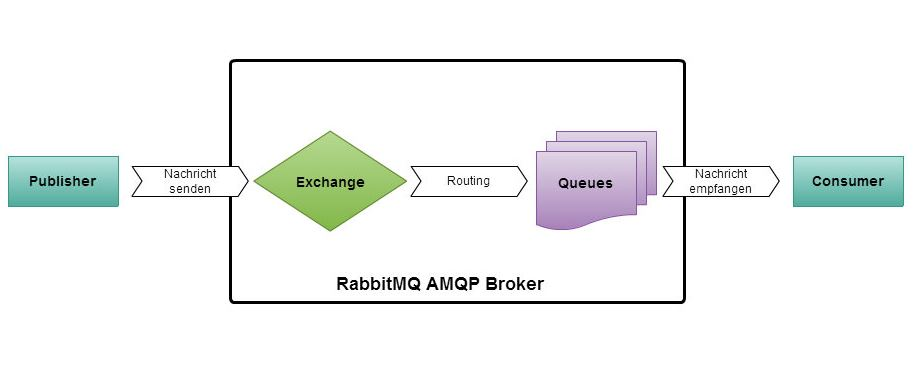
\includegraphics[width=13cm, trim={0cm 1.3cm 0cm 0.8cm}]{img/rabbitmq.jpg}
	\caption{RabbitMQ als Message-Broker, Quelle: \cite{rabbit}}
	\label{fig:rabbit}
\end{figure}

\noindent
Abbildung \ref{fig:rabbit} skizziert den Aufbau des \textit{Message-Brokers}. Der \textit{Publisher} ist dabei der \textit{Workload-Service} und der \textit{Consumer} der Microservice auf der \textit{Bosch IoT Cloud}, in dem der \textit{Python-Consumer} die Jobs verarbeitet. \\
Das CPU-Monitoring verhält sich wie folgt: Alle 10-15 Sekunden stehen pro Microservice-Instanz ein CPU-Update bereit. Daher ist die Auslastung zu Beginn nicht sofort auf 100\%, sondern erst nach 10 Sekunden auf 50\% und kurze Zeit später bei 100\% , auch wenn die Instanz bereits unter Volllast läuft. Erst nach ca. 20 Sekunden erhält man also die erste richtige Messung bei einer neuen Instanz. Dies ist deutlich anhand der gemessenen Werte (vgl. Abbildung \ref{fig:cpuResult}) erkennbar. Bei der Warteschlange wird ca. alle 5 Sekunden ein Update gemacht. \\
Basierend auf diesen Informationen wurden die Konfigurationsparameter erhoben. Nicht-spezifizierte oder nur implizit gegebene Parameter wurden geschätzt. Das genaue Anpassen aller Parameter ist jedoch nicht Teil des Praktikums, muss aber bei einer zielgenaueren Evaluation eines Auto-Skalierers gewissenhaft erledigt werden.




\section{Evaluationsergebnisse}
Die Abbildungen \ref{fig:vmsResult}, \ref{fig:cpuResult}, \ref{fig:queueLength} und \ref{fig:queueArrival} vergleichen die simulierten Werte (linke Spalte) mit der real gemessenen (rechte Spalte). Die Werte der jeweiligen Diagramme werden alle über die Zeit (x-Achse) aufgetragen. Die Einheit bei den Simulationsergebnissen ist über die Intervallnummer gegeben, die bei der realen Messung in Sekunden. 
Das Diagramm in Abbildung \ref{fig:vmsResult} beschreibt die Anzahl virtueller Maschinen über die Zeit. Es ist deutlich zu sehen, dass der Autoskalierer mit den simulierten Metriken, nahezu die selben Skalier-Entscheidungen trifft. \\
In Abbildung \ref{fig:cpuResult} wird die CPU-Auslastung aufgetragen. Auch hier stimmen die Simulationsergebnisse ziemlich genau mit der Realität überein. Wie in Sektion \ref{sec:Evaluation:Aufbau} beschrieben, weichen die ersten 20 Sekunden der real gemessenen Werte von der tatsächlichen Auslastung ab. Deshalb sind die simulierten Ergebnisse an dieser Stelle überraschenderweise sogar deutlich genauer. \\




%"l, b, r, t"
\begin{figure}[!h]
	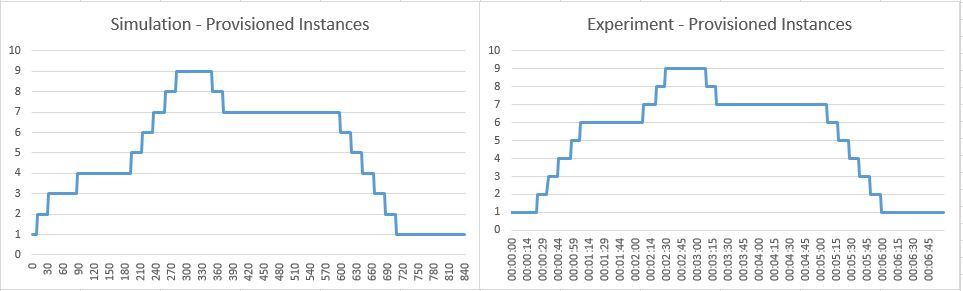
\includegraphics[width=\textwidth, trim={0cm 0cm 0cm 0cm}]{img/vms.jpg}
	\caption{Vergleich der Menge an Virtuellen Maschinen}
	\label{fig:vmsResult}
\end{figure}

%"l, b, r, t"
\begin{figure}[!h]
	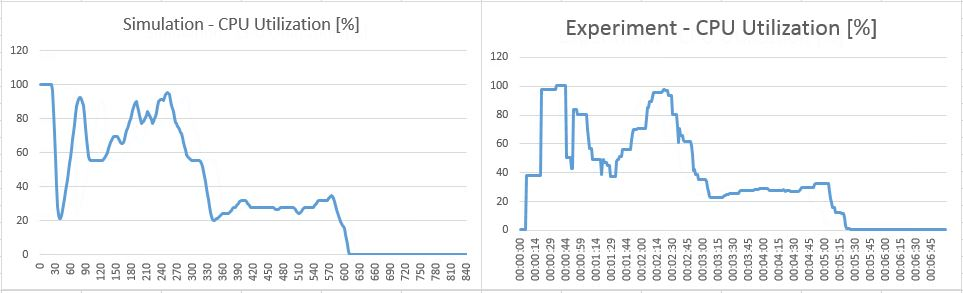
\includegraphics[width=\textwidth, trim={0cm 0cm 0cm 0cm}]{img/cpu.jpg}
	\caption{Vergleich der CPU Auslastung}
	\label{fig:cpuResult}
\end{figure}

\noindent
Das Diagramm in Abbildung \ref{fig:queueLength} vergleicht die simulierte und die tatsächliche Warteschlangen-Länge. Hier weichen die Simulationsergebnisse von der Realität ab. Dies liegt vor allem an der CPU: Da bei der realen Infrastruktur langsamer gemessen wird, werden vom Auto-Skalierer verzögerte Ressourcen provisioniert, wodurch die Warteschlangenlänge in der Realität schneller ansteigt.
. Dennoch ist die auch in der Simulation an den Ausschlägen zu erkennen, wann die Kapazität der Infrastruktur nicht ausreichend für die anliegende Last ist.\\
Ankunfts-und Verarbeitungsrate (Abbildung \ref{fig:queueArrival}) der Simulation stimmen hingegen mit der Realität relativ genau überein. Die Ankunftsrate (blaue Linie) der Simulation ist bis auf wenige nicht vorhandenen  Ausschläge ähnlich. Die Glättung der Kurve in der Simulation ist ein Effekt der Mittelwertbildung. 



%"l, b, r, t"
\begin{figure}[!h]
	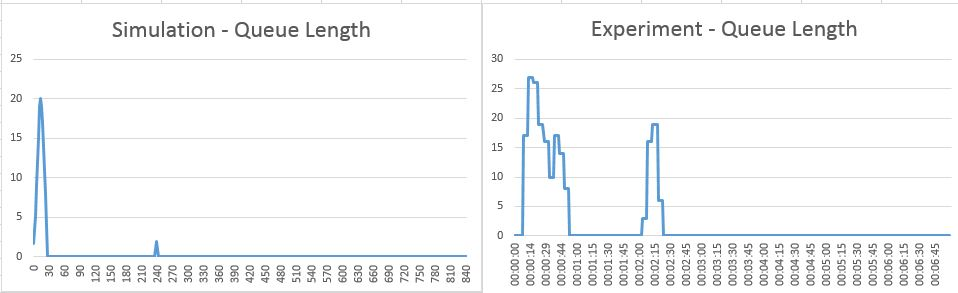
\includegraphics[width=\textwidth, trim={0cm 0cm 0cm 0cm}]{img/queueLength.jpg}
	\caption{Evaluationsergebnisse der Warteschlangenlänge}
	\label{fig:queueLength}
\end{figure}

%"l, b, r, t"
\begin{figure}[!h]
	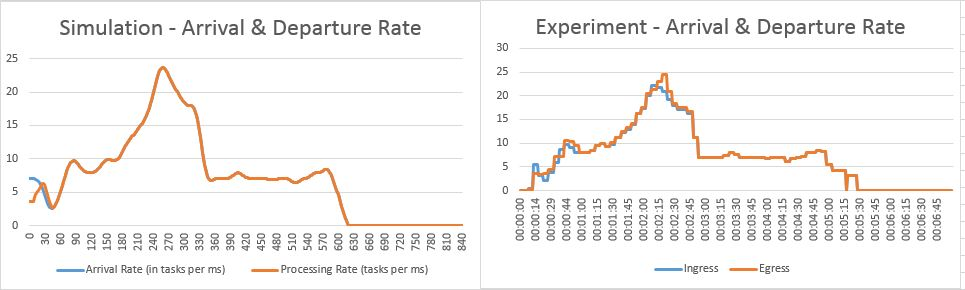
\includegraphics[width=\textwidth, trim={0cm 0cm 0cm 0cm}]{img/queueArrival.jpg}
	\caption{Evaluationsergebnisse der Ankunfts- und Verarbeitungszeit der Warteschlange}
	\label{fig:queueArrival}
\end{figure}



\section{Limitierungen}
Wie die Simulationsergebnisse zeigen, stimmen die Werte nicht zu 100\% mit der Realität überein. Dies ist der Tatsache geschuldet, dass die Parameter der Testbench nie genau bestimmt werden können. Beispielsweise wird vorausgesetzt, dass eine Virtuelle Maschine immer eine feste Zeit brauch, um ein Paket abzuarbeiten. VMs selbst sind aber auch nur eine weitere Abstraktion einer darunterliegenden Hardware-oder Software-Schicht, weshalb diese Annahme im Allgemeinen nicht gilt, denn die Verarbeitung eines Tasks kann durch eine darunterliegende Schicht pausiert werden. \\
Ein weiterer Grund ist die Umrechnung der externen Einheit [ms] auf die interne Einheit [Intervall], die oftmals mit Rundungsfehler behaftet ist. Dies ist insbesondere dann der Fall, wenn die Konfigurationsparameter nicht als Vielfache der Auflösung angegeben werden. Zwar mindert die interne Skalierung Rundungsfehler, kann sie aber nicht gänzlich eliminieren. \\
Ein weiterer Nachteil der aktuellen Implementierung ist die Gleichbehandlung aller Jobs. Es wird die vereinfachte Annahme gemacht, dass eine VM jeden Job in gleicher Zeit verarbeiten kann, was allerdings nicht der Realität entspricht. \\
Im Allgemeinen können viele Parameter nicht eindeutig bestimmt werden, da diese entweder nicht genau bekannt sind, oder aber nicht konstant sind.



\section{Zusammenfassung und Ausblick}
Das Ziel dieses Praktikums war es, eine Testbench zur Evaluation von Autoskalierern zu Entwickeln. Dafür wurde eine zeit-diskrete Simulations-Engine implementiert, die eine Cloud-Infrastruktur abstrahiert. Die wichtigsten Komponenten der Engine sind i) das \textit{InfrastructureModel}, das die Virtuellen Maschinen verwaltet und somit die Abarbeitung der Jobs simuliert ii) das \textit{QueueModel}, das eine Warteschlange darstellt, die sowohl ein Verzögerungsglied, wie auch ein Pufferspeicher simuliert iii) die \textit{MetricSource} als Komponente, die Metriken für einen Auto-Skalierer bereitstellt iv) ein Tracking-Mechanismus, der zeit-diskret die Informationen aller Komponenten abspeichert. Ein Auto-Skalierer ist ebenfalls Teil des Projektes, ist aber streng genommen kein Teil der Testbench, sondern wird nur über Schnittstellen an diese angebunden. \\
Nach der Implementierung der Applikation wurde ein Experiment durchgeführt. Dazu wurde eine spezifizierte Workload auf einer realen Infrastruktur getestet. Diese Infrastruktur wurde durch einen Auto-Skalierer dynamisch adaptiert, es wurden also je nach Last Virtuelle Maschinen instanziiert oder heruntergefahren. Das Verhalten der realen Komponenten ist dabei aufgezeichnet worden. Anschließend sind die Parameter der Infrastruktur und des Auto-Skalierers bestmöglich approximiert worden. Diese wurden als Eingabe-Konfiguration in die Testbench gegeben. Ebenso wurde die verwendete Workload als Eingabe verwendet. Die zu simulierende Zeit betrug 7 Minuten. Die Simulationszeit wenige Sekunden. \\
Der Vergleich der realen und der simulierten Ergebnisse ist höchst zufriedenstellend. Angemerkt werden sollte noch, dass die Simulation selbst in nur wenigen Sekunden durchgeführt werden konnte. Projiziert man dies auf ein deutlich längeres Intervall eines realen Experiments, so ist der Nutzen dieser Simulation deutlich absehbar. Weiterhin mussten für die Simulation keine Ressourcen einer Cloud-Infrastruktur genutzt werden, sondern lediglich ein Desktop-Rechner, auf dem diese durchgeführt wurde. \\
Für die Zukunft wäre es denkbar, ein geeignetes Frontend zu implementieren, sodass die Durchführung der Simulation benutzerfreundlicher ist. Vor allem die händische Eingabe der Parameter, beziehungsweise das (noch) etwas umständliche Anbinden eines anderen Auto-Skalierers kann durch eine geeignete Benutzeroberfläche deutlich erleichtert werden.

















%% --------------------
%% |   Bibliography   |
%% --------------------

%% Add entry to the table of contents for the bibliography
\printbibliography[heading=bibintoc]

%% ----------------
%% |   Appendix   |
%% ----------------
\appendix
%% LaTeX2e class for student theses
%% sections/apendix.tex
%% 
%% Karlsruhe Institute of Technology
%% Institute for Program Structures and Data Organization
%% Chair for Software Design and Quality (SDQ)
%%
%% Dr.-Ing. Erik Burger
%% burger@kit.edu
%%
%% Version 1.3.3, 2018-04-17

\iflanguage{english}
{\chapter{Appendix}}    % english style
{\chapter{Anhang}}      % german style
\label{ch:appendix}


%% -------------------
%% | Example content |
%% -------------------
\section{BPMN Models}
\label{sec:appendix:BPMN Models}








\end{document}
